\documentclass{article}
\usepackage{amssymb}
\usepackage{graphicx}

\documentclass{article}
\usepackage{arxiv}
\usepackage{float}
\usepackage[utf8]{inputenc} % allow utf-8 input
\usepackage[T1]{fontenc}    % use 8-bit T1 fonts
\usepackage{hyperref}       % hyperlinks
\usepackage{url}            % simple URL typesetting
\usepackage{booktabs}       % professional-quality tables
\usepackage{amsfonts}       % blackboard math symbols
\usepackage{nicefrac}       % compact symbols for 1/2, etc.
\usepackage{microtype}      % microtypography
\usepackage{lipsum}

\title{Bayesian Methods Project Report \\
Based on Improving MCMC by Proposal Learning}


\author{
  Anastasiia Baiandina
   \And
 Kristina Rakova
}

\begin{document}
\maketitle

\begin{abstract}
In the paper, the authors propose the generalization of Hamiltonian Monte Carlo method parametrized by deep neural networks. The authors claim to have improved mixing speed by maximization of expected squared jumped distance. They compare their results with vanilla HMC. In the project, we build their model and reproduce their experiments.
\end{abstract}


\section*{Hamiltonian Monte Carlo}
Let $p$ be the target distribution analytically known over $\mathcal{X}$. The goal is to provide samples from $p$. Obtaining samples corresponds to constructing a Markov Chain, whose stationary distribution is $p$. Given any proposal distribution $q$, satisfying mild conditions, we can construct a transition kernel that forms the desired Markov Chain.

In HMC, it is assumed that $p(x)$ is defined by an energy function $U(x)$, $p(x) \propto \exp \{ U(x) \}$, where the state $x \in \mathbb{R}^n$. HMC extends the state space with an additional momentum vector $v \in \mathbb{R}^n$, where $v$ is distributed independently from $x$, as $p(v) \propto \exp \{-\frac{1}{2} v^T v\}$. From an augmented state $\xi \triangleq (x, v)$, HMC produces a proposed state $\xi' = (x', v')$ by approximately integrating Hamiltonian dynamics jointly on $x$ and $v$, with $U(x)$ taken to be the potential energy, and $\frac{1}{2} v^T v$ the kinetic energy.

The dynamics are typically simulated using the leapfrog integrator
\[
    \mathbf{L}\xi \triangleq \mathbf{L}(x, v) \triangleq (x', v')
\]
\begin{eqnarray*}
v^{1/2} = & v - \frac{\varepsilon}{2} \partial_x U(x) \\
x' = & x + \varepsilon v^{1/2} \\
v' = & v - \frac{\varepsilon}{2} \partial_x U(x')
\end{eqnarray*}
and the momentum flip operator
\[
    \mathbf{F}(x, v) \triangleq \mathbf{F}(x, -v).
\]

The important property is that the transformation $\mathbf{FL}$ is volume-preserving. Moreover, the determinant of the Jacobian of this transformation equals to $1$. Leaving it in symbolic form, the acceptance probability can be written as
\[
    A(\mathbf{FL}\xi | \xi) = \min \Big( 1, \frac{p(\mathbf{FL}\xi)}{p(\xi)} \Big| \frac{\partial [\mathbf{FL}\xi]}{\partial \xi^T} \Big| \Big).
\]


\section*{L2HMC}

In the proposed method, the authors introduce the new binary direction variable $d \sim \mathrm{Uniform}\{-1, 1\}$, and $\xi \triangleq (x, v, d)$, $p(\xi) = p(x)p(v)p(d)$. To each step $t$ of the updates, a fixed random binary mask $m_t \in \{0, 1\}^n$ is assigned, which will determine which variables are affected by each sub-update.

The update steps are
\begin{eqnarray*}
        \zeta_1 \triangleq (x, \partial_x U(x), t), & v' = v \odot \exp \big\{ \frac{\varepsilon}{2} S_v(\zeta_1) \big\} - \frac{\varepsilon}{2} \Big( \partial_x U(x) \odot \exp \big\{ \varepsilon Q_v(\zeta_1) \big\} + T_v(\zeta_1) \Big) \\
        \zeta_2 \triangleq (x_{\bar{m}^t}, v, t), & x' = x_{\bar{m}^t} + m^t \odot \Big[ x \odot \exp \big\{ \varepsilon S_x(\zeta_2) \big\} + \varepsilon \Big( v' \odot \exp \big\{ \varepsilon Q_x(\zeta_2) \big\} + T_x(\zeta_2) \Big) \Big] \\
        \zeta_3 \triangleq (x'_{m^t}, v, t), & x'' = x'_{m^t} + \bar{m}^t \odot \Big[ x' \odot \exp \big\{ \varepsilon S_x(\zeta_3) \big\} + \varepsilon \Big( v' \odot \exp \big\{ \varepsilon Q_x(\zeta_3) \big\} + T_x(\zeta_3) \Big) \Big] \\
        \zeta_4 \triangleq (x'', \partial_x U(x''), t), & v'' = v' \odot \exp \big\{ \frac{\varepsilon}{2} S_v(\zeta_4) \big\} - \frac{\varepsilon}{2} \Big( \partial_x U(x'') \odot \exp \big\{ \varepsilon Q_v(\zeta_4) \big\} + T_v(\zeta_4) \Big)
    \end{eqnarray*}
    
If assume $S, Q, T \equiv 0$, then we get the vanilla HMC. $S, Q, T$ are neural networks with 2 hidden layers with 10 units and ReLU non-linearities. We train with Adam optimizer 5000 iterations with exponential decay learning rate.

To give intuition into these terms, the scaling applied to the momentum can enable, among other things, acceleration in low-density zones, to facilitate mixing between modes. The scaling term applied to the gradient of the energy may allow better conditioning of the energy landscape (e.g., by learning a diagonal inertia tensor), or partial ignoring of the energy gradient for rapidly oscillating energies.

To model L2HMC transitions, we define the three operators: leapfrog operator $\mathbf{L}_{\theta}\xi = \mathbf{L}_{\theta}(x, v, d) = (x''^{\times M}, v''^{\times M}, d)$; flip operator $\mathbf{F}\xi = \mathbf{F}(x, v, d) = (x, v, -d)$; re-sampling operator $\mathbf{R}\xi = \mathbf{R}(x, v, d) = (x, v', d')$, where $v' \sim \mathcal{N}(o, I)$, $d' \sim \mathrm{Uniform}\{-1, 1\}$. Then, the sampling is as follows:
\begin{enumerate}
    \item $\xi' = \mathbf{FL}_{\theta}\xi$ with probability $A(\mathbf{FL}\xi | \xi)$, otherwise $\xi' = \xi$;
    \item $\xi' = \mathbf{R}\xi$.
\end{enumerate}

Define $\delta(\xi', \xi) = \delta((x, v, d), (x', v', d')) = \| x - x' \|_2^2$. The aim is to maximize the expected jumped distance $\mathbb{E}_{p(\xi)} \big[ \delta (\mathbf{FL}_{\theta}\xi, \xi) A(\mathbf{FL}_{\theta}\xi, \xi) \big]$. However, this loss need not encourage mixing across the entire state space. Maximizing this objective can lead to regions of state space where almost no mixing occurs, so long as the average squared distance traversed remains high. To optimize both for typical and worst case behavior, the authors include a reciprocal term in the loss
\[
    \ell_{\lambda}(\xi, \xi', A(\xi' | \xi)) = \frac{\lambda^2}{\delta(\xi, \xi')A(\xi' | \xi)} - \frac{\delta(\xi, \xi')A(\xi' | \xi)}{\lambda^2},
\]
where $\lambda$ is a scale parameter. The second term encourages typical moves to be large, while the first term strongly penalizes the sampler if it is ever in a state where it cannot move effectively $-\delta(\xi', \xi)$ being small resulting in a large loss value. The sampler is trained by minimizing this loss over both the target distribution and initialization distribution:
\[
    \mathcal{L}(\theta) = \mathbb{E}_{p(\xi)} \big[ \ell_{\lambda}(\xi, \mathbf{FL}_{\theta}\xi, A(\mathbf{FL}_{\theta}\xi | \xi)) \big] + \lambda_b \mathbb{E}_{q(\xi)} \big[ \ell_{\lambda}(\xi, \mathbf{FL}_{\theta}\xi, A(\mathbf{FL}_{\theta}\xi | \xi)) \big].
\]

The parameter $\lambda_b$ controls the strength of the ‘burn-in’ regularization.














\section*{Expriments}

\subsection*{Toy Distributions}

We compared the performance of L2HMC with HMC on several 2-dimensional distributions. The large difference in sampling they showed on strongly correlated Gaussian, with $\mu = (0, 0)^T$ and $\Sigma = [[50.05, -49.95], [-49.95, 50.05]]$. For L2HMC, the sampling is much more uniform than for HMC that is concentrated only on the central part of the distribution.

\begin{figure}[H]
\centering
\begin{minipage}{.5\textwidth}
  \centering
  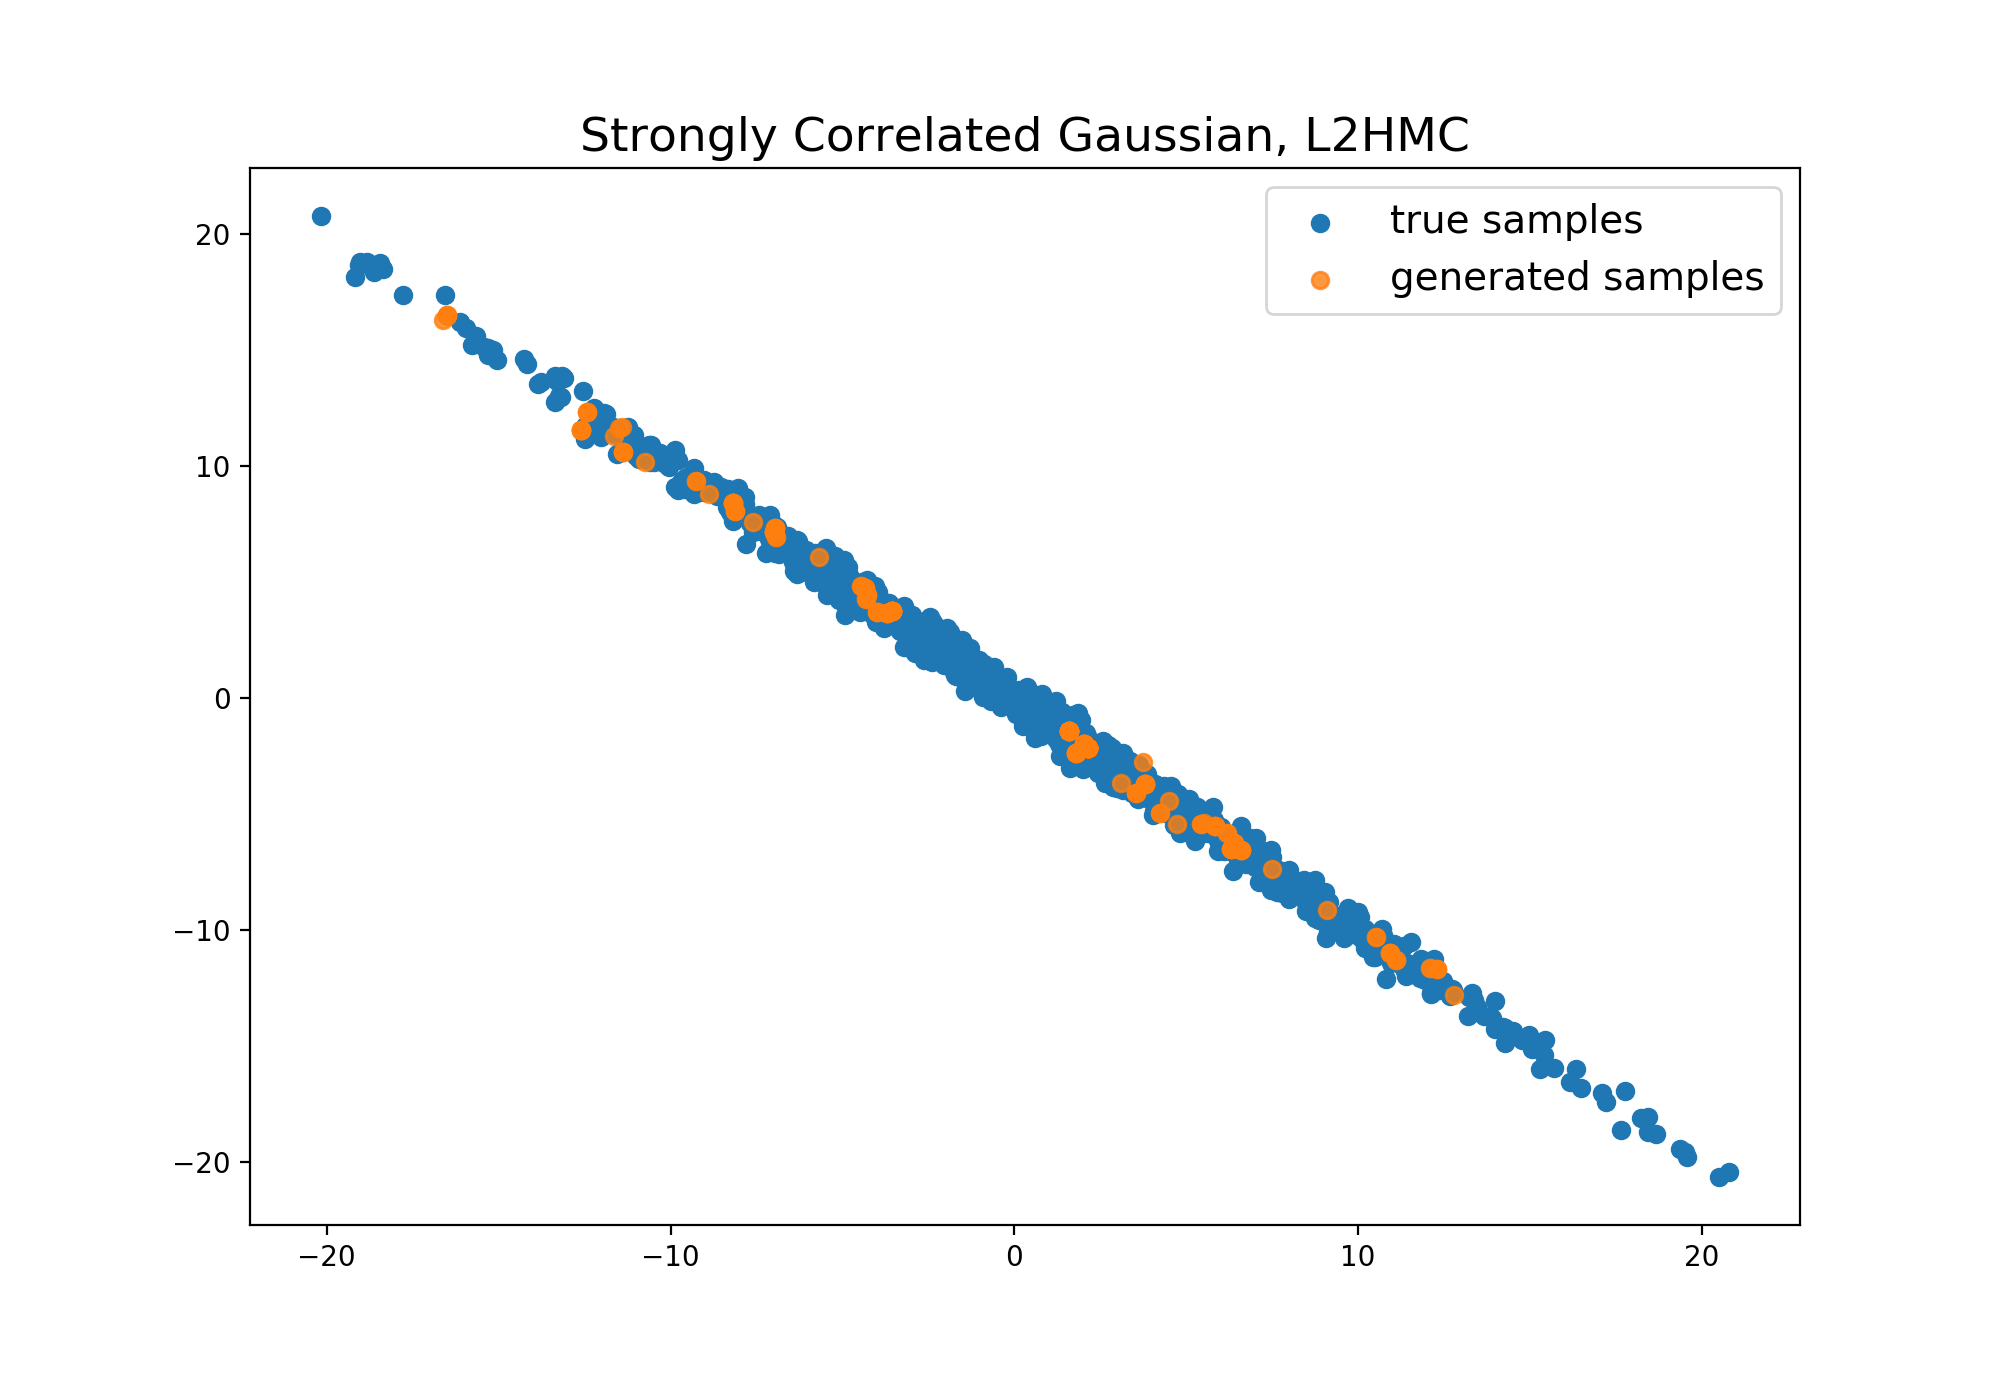
\includegraphics[width=\linewidth]{Strongly_Correlated_Gaussian_L2HMC.png}
  %\captionof{figure}{A figure}
  %\label{fig:test1}
\end{minipage}%
\begin{minipage}{.5\textwidth}
  \centering
  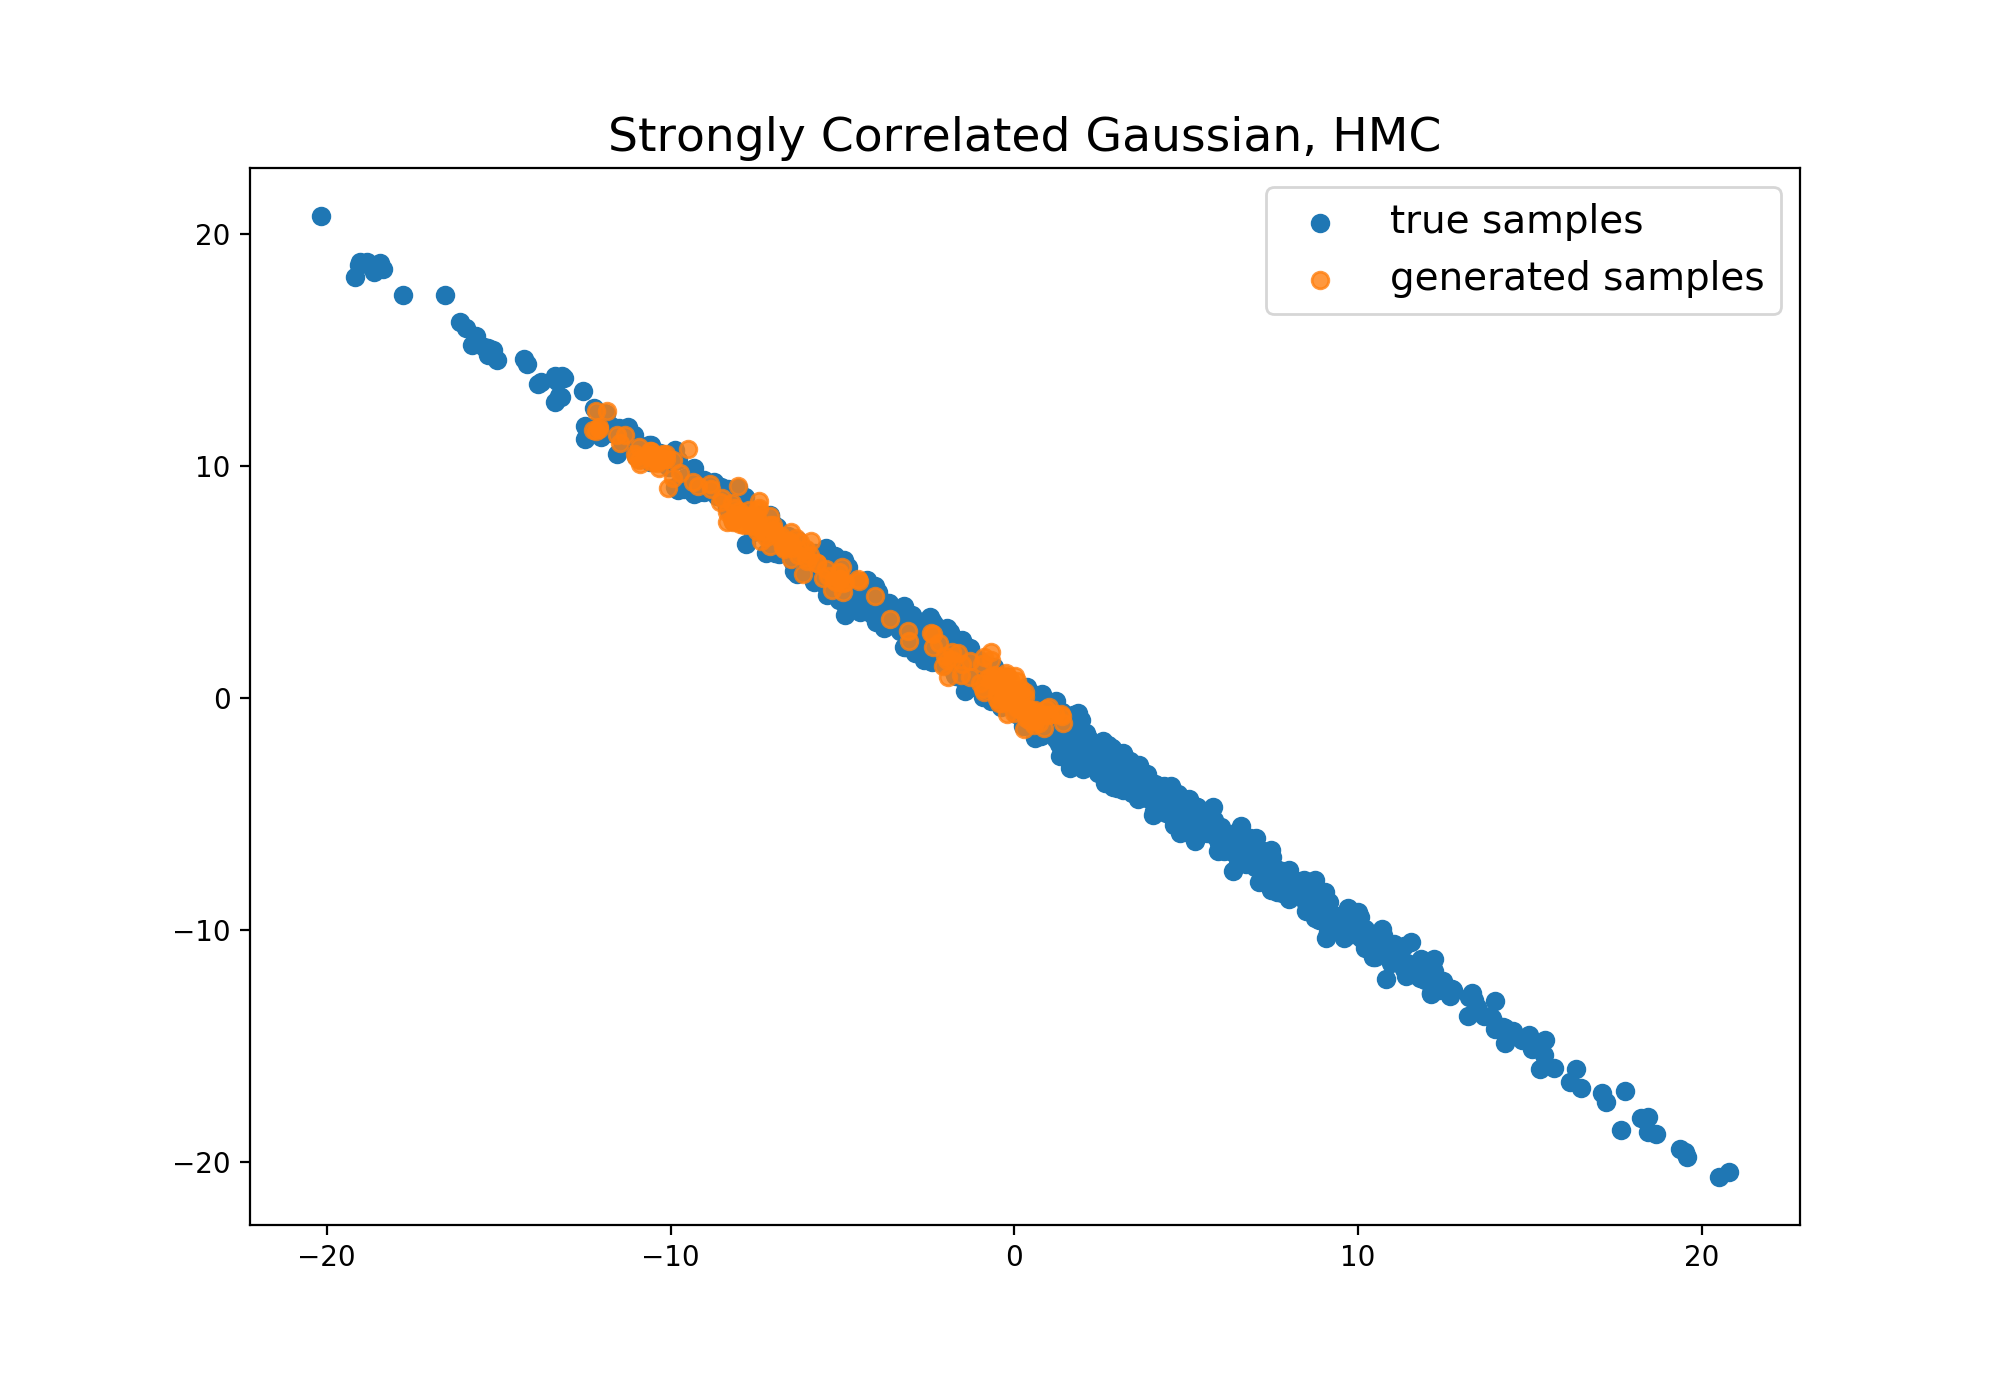
\includegraphics[width=\linewidth]{Strongly_Correlated_Gaussian_HMC.png}
  %\captionof{figure}{Another figure}
  %\label{fig:test2}
\end{minipage}
\end{figure}

The interesting difference can be seen for the mixture of Gaussians. While HMC is unable to jump between the modes of the distribution, the L2HMC can sample from the both if them.

\begin{figure}[H]
\centering
\begin{minipage}{.5\textwidth}
  \centering
  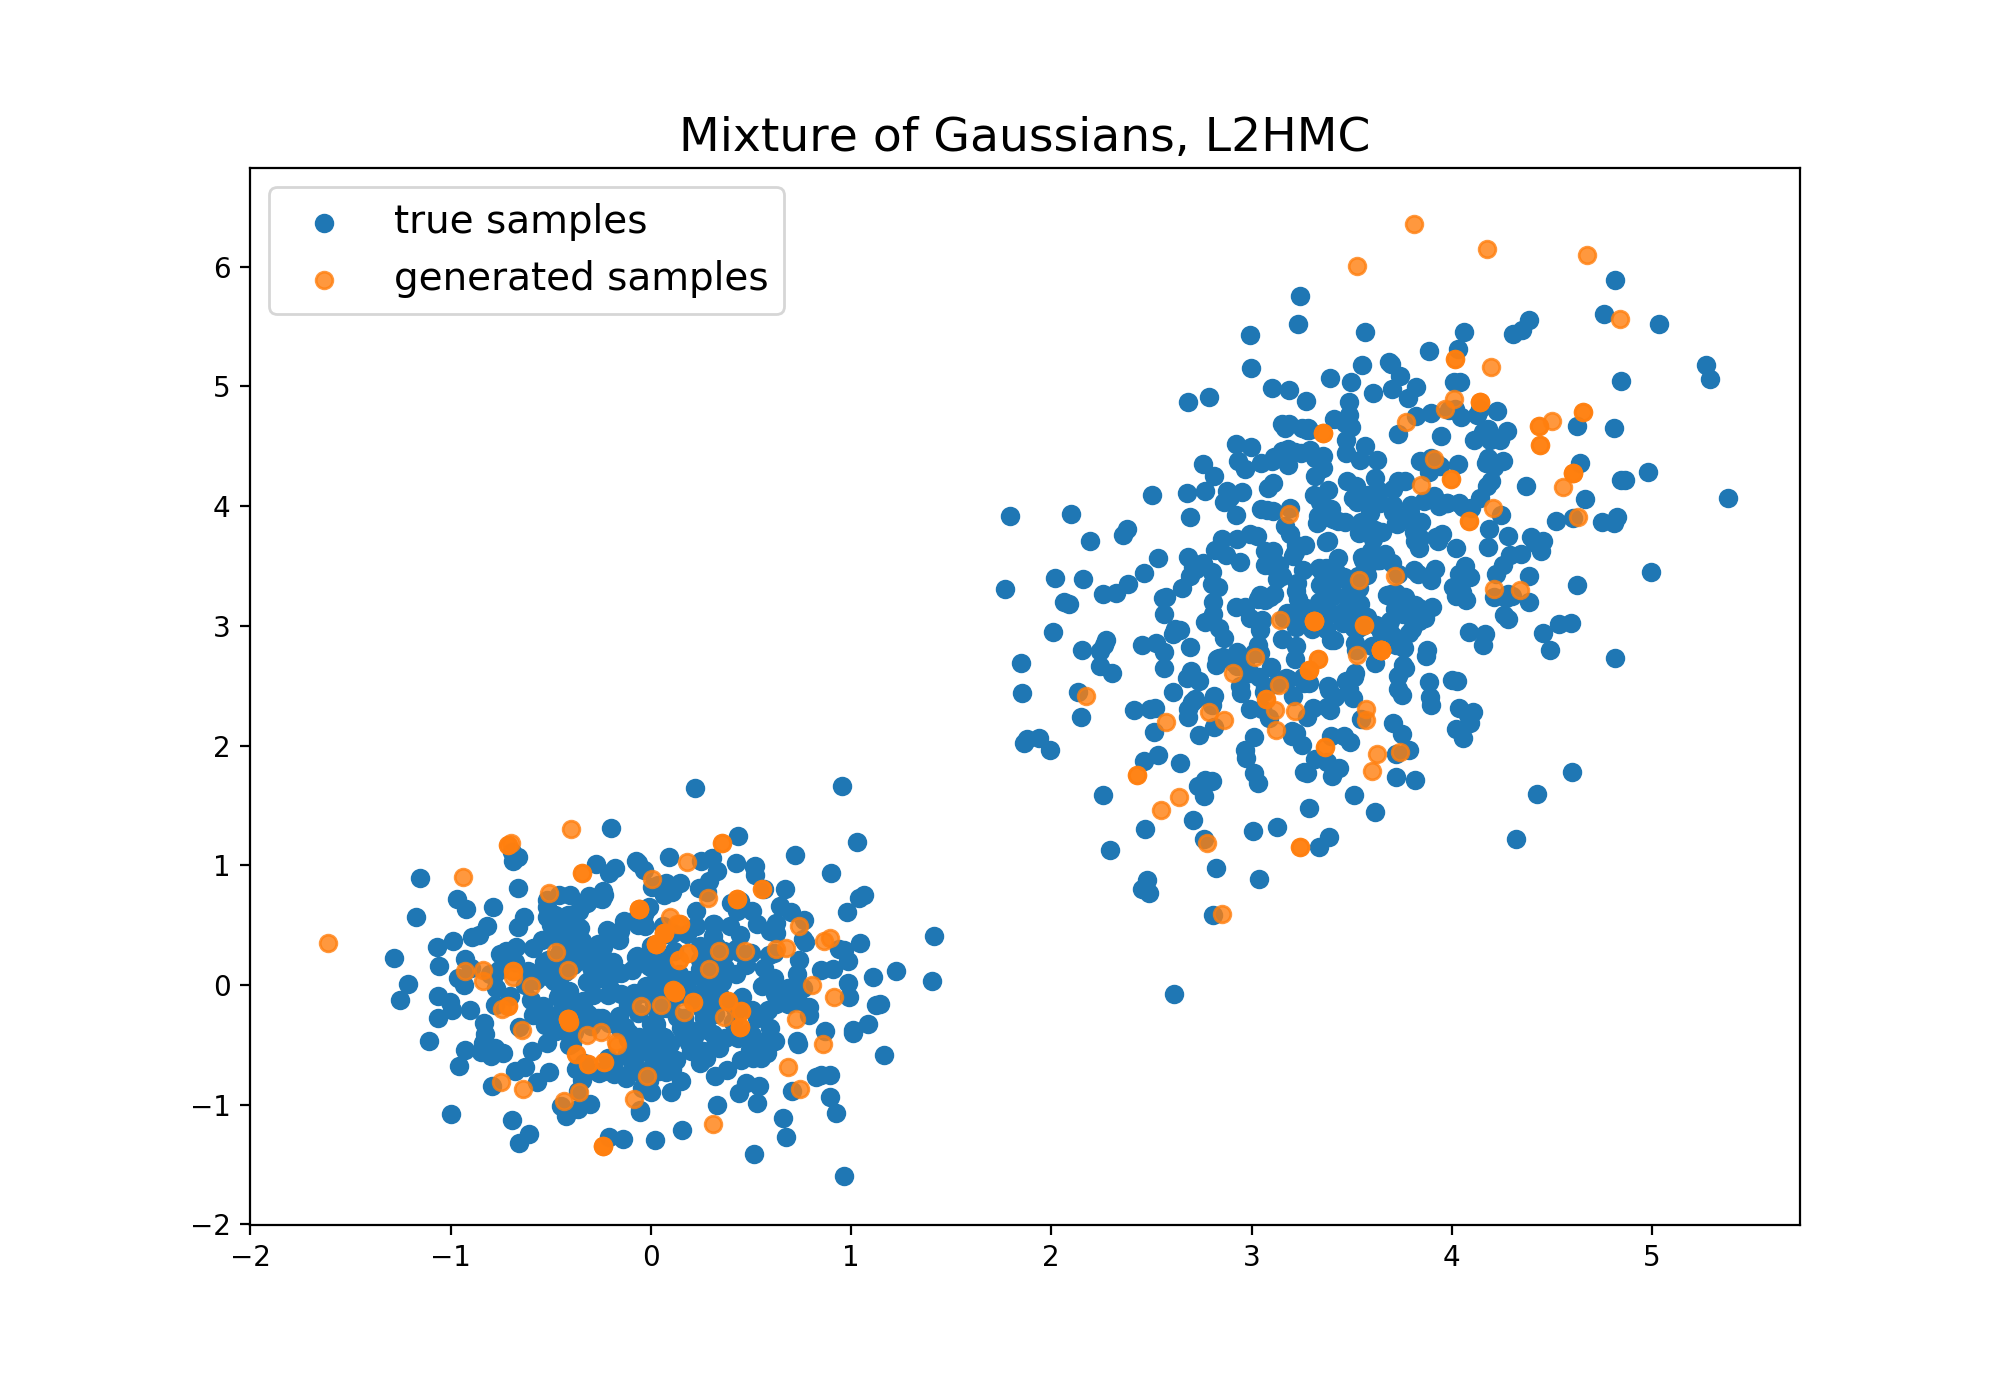
\includegraphics[width=\linewidth]{Mixture_of_Gaussians_L2HMC.png}
  %\captionof{figure}{A figure}
  %\label{fig:test1}
\end{minipage}%
\begin{minipage}{.5\textwidth}
  \centering
  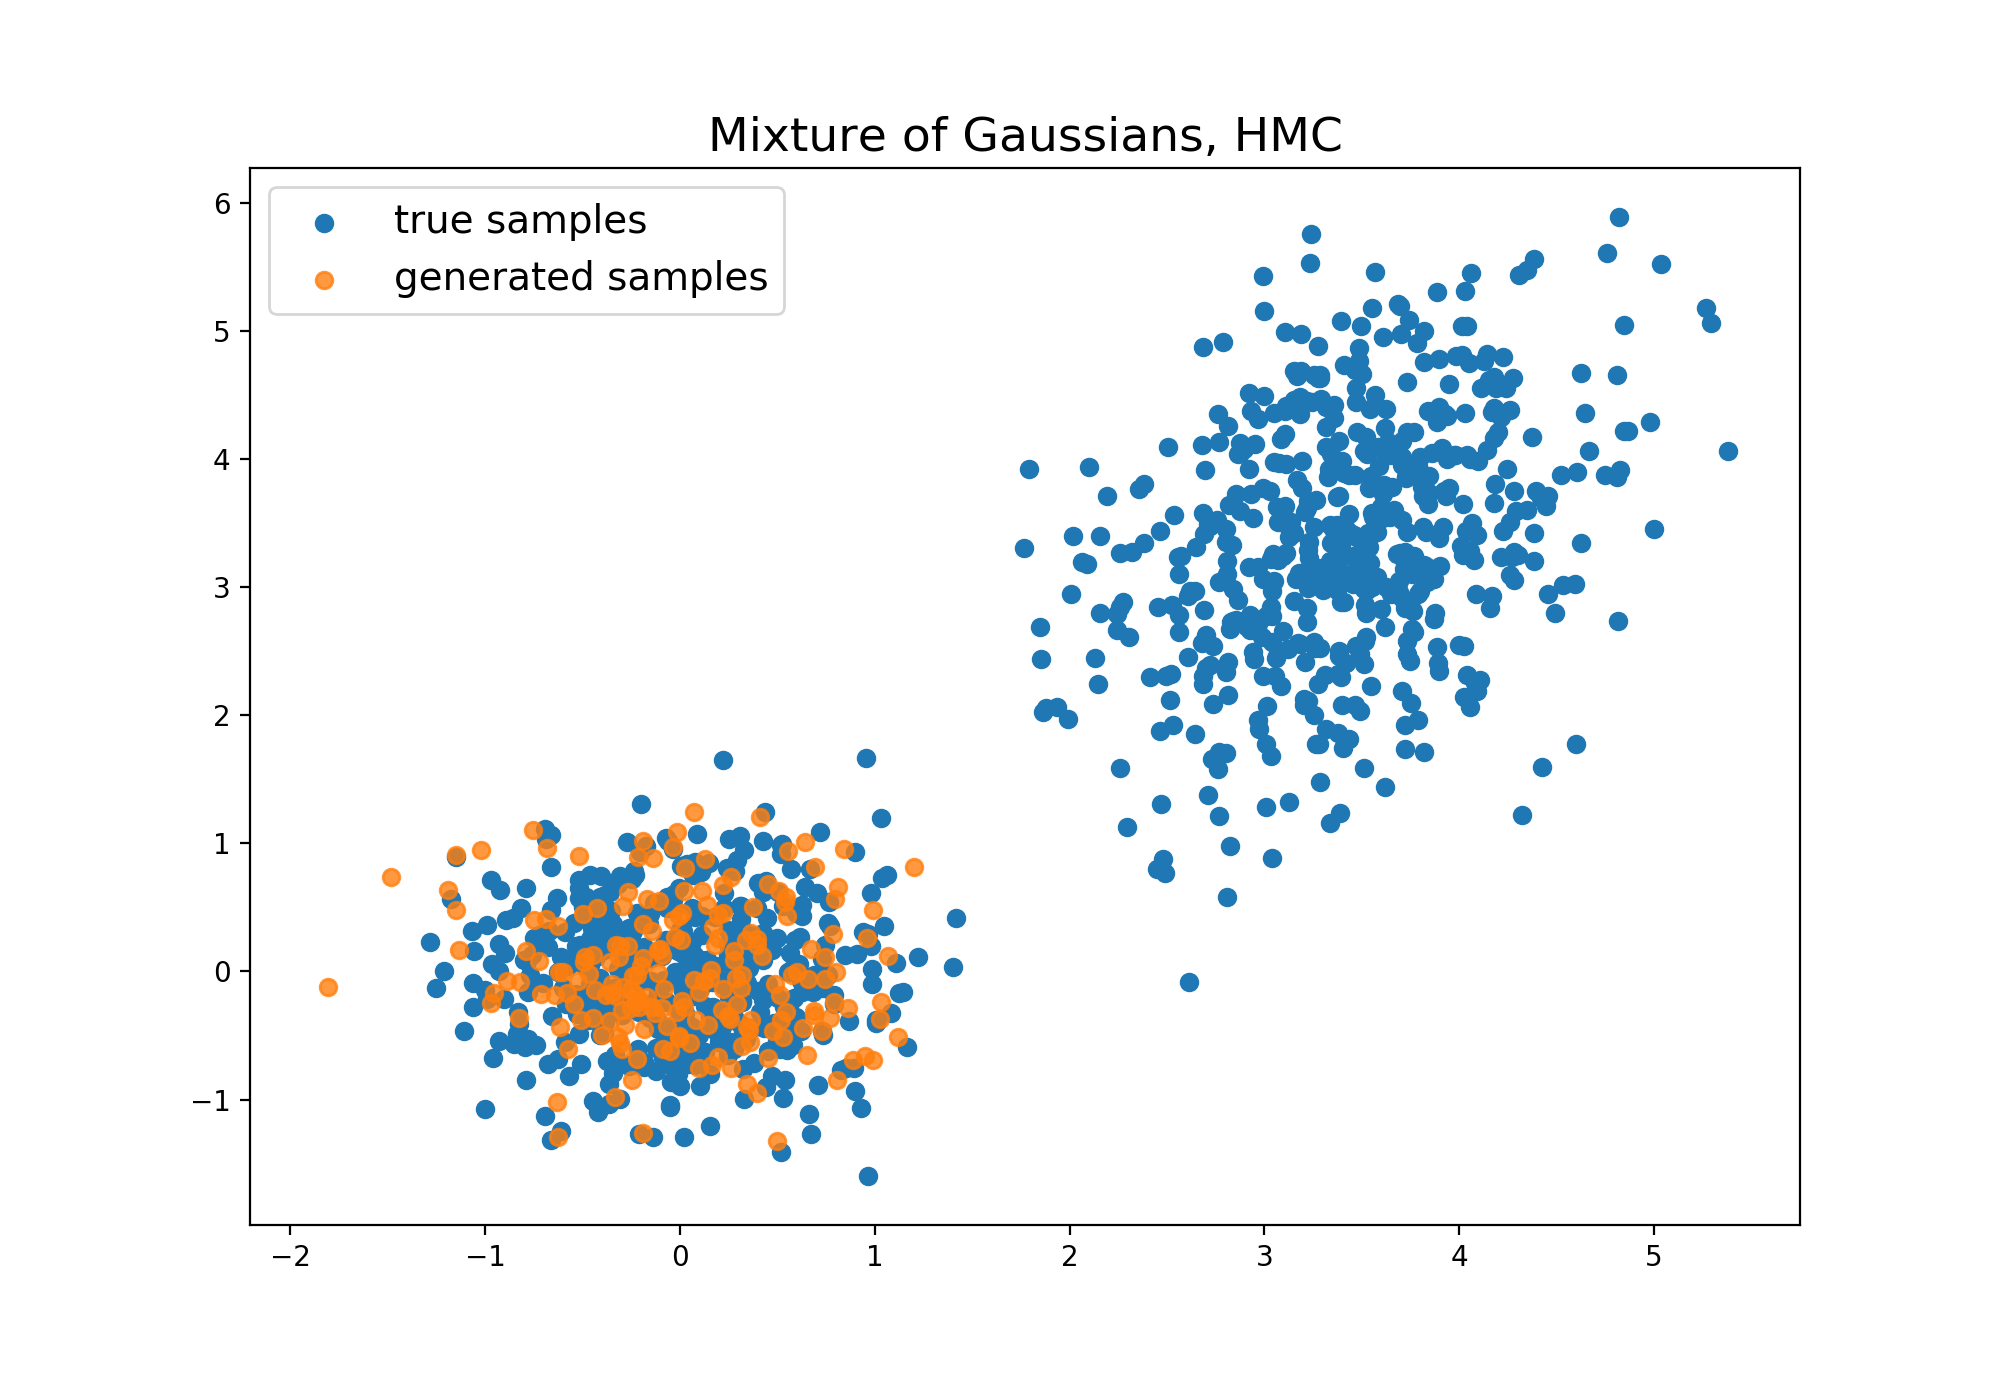
\includegraphics[width=\linewidth]{Mixture_of_Gaussians_HMC.png}
  %\captionof{figure}{Another figure}
  %\label{fig:test2}
\end{minipage}
\end{figure}

For $S, T, Q$ there are the neural networks with the two hidden layers with 10 hidden units and ReLU activations. It was trained with Adam with exponentially decaying learning rate. We train for 5000 iterations with a batch size of 200.



\subsection*{MNIST}
We apply learned sampler to the task of training, and sampling from the posterior of a latent  variable model. Given a family of parametric decoders {$z \rightarrow p(x|z, \phi), \phi \in \Phi$}, and a dataset $D$ we want to find optimal $\phi^*$. For vanilla VAE this can be done by maximizing tractable lower-bound on the log-likelihood:
$$L_{ELBO}(x,\phi, \psi) = \mathbb{E}_{q_{\psi}(z|x)}\left[p(x|z,\phi)\right]-KL(q_{\psi}(z|x)||p(z)),$$
where $q_{\psi}(z|x)$ is typically parametrized by Neural Network. We want to improve such model and embedd L2HMC to VAE pipeline to obtain more exact posterior samples from  $p(x|z)$. After obtaining sample from approximate posterior $q_{\psi}(z|x^i)$, we define energy function $U(z, x^i) = -\log p(z)-\log p(x^i|z, \phi)$. Then using L2HMC we sample latent variable $z'$ from 
distribution with energy function $U(z, x^i)$. After that we maximize log-likelhood $\log p(x^i|z', \phi)$ and ELBO. Such transformation of algorithm improves the efficiency of posterior sampler.

The decoder $p_{\phi}$ is a neural network with 2 fully connected layers, with 1024 units each and softplus non-linearities, and outputs Bernoulli activation probabilities for each pixel. The encoder  $q_{\psi}$ has the same architecture, returning mean and variance for the approximate posterior. Our model was trained for 100 epochs with Adam optimizer and a learning rate $10^{-3}$. $S, Q, T$ are neural networks with 2 hidden layers with 200 units and ReLU non-linearities.

In Figure \ref{fig:vae}, we can see generated samples using Vanilla VAE and L2HMC VAE. It can be noticed that decoder, training with L2HMC produces sharper samples than the Vanilla. 

\begin{figure}[H]
  \centering
  \begin{minipage}[b]{0.45\linewidth}
    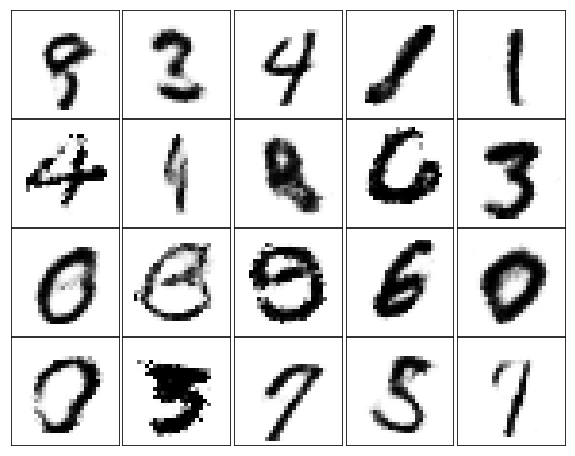
\includegraphics[width=\linewidth]{vanilla_vae.png}
    \caption{Vanilla VAE}
  \end{minipage}
  \begin{minipage}[b]{0.45\linewidth}
    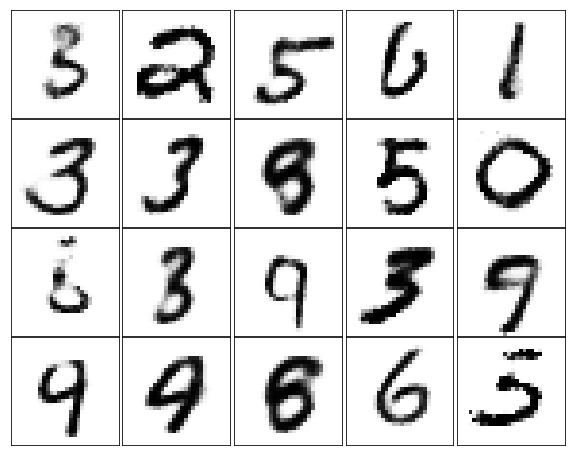
\includegraphics[width=\linewidth]{l2hmc_vae.png}
    \caption{L2HMC VAE}
  \end{minipage}
  \label{fig:vae}
  \caption{Generated samples}
\end{figure}

After training L2HMC parameters we can compare mixing property of model with HMC, generating long chains of samples. As we can see in fig\ref{fig:aut} L2HMC generates new uncorrelated sample faster that HMC with different parameters.
\begin{figure}[H]
    \centering
 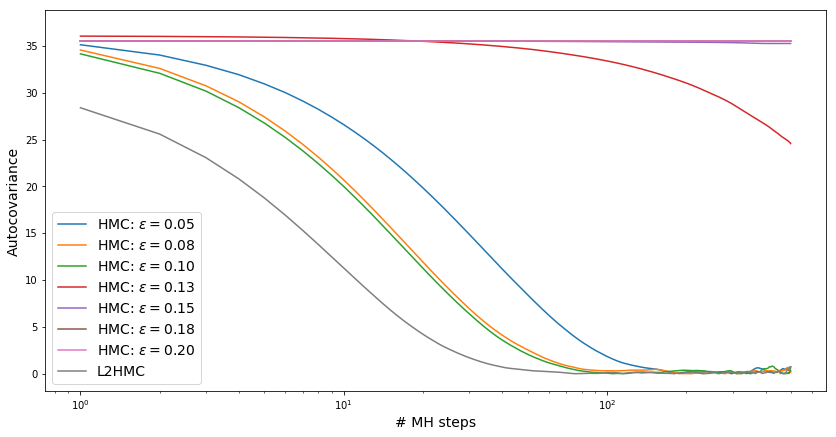
\includegraphics[width=0.8\linewidth]{autocovariance.png}
    \caption{Autocovariance}
    \label{fig:aut}
\end{figure}

\begin{thebibliography}{}
\bibitem{}
Levy D., Hoffman M. D., Sohl-Dickstein J. Generalizing Hamiltonian Monte Carlo with Neural Networks //arXiv preprint arXiv:1711.09268. – 2017.
\end{thebibliography}

\end{document}
